\documentclass[brazil]{beamer}
\usepackage[brazilian]{babel}
\usepackage[utf8]{inputenc}

\usepackage{fancyvrb}
\usepackage{color}



\makeatletter
\def\PY@reset{\let\PY@it=\relax \let\PY@bf=\relax%
    \let\PY@ul=\relax \let\PY@tc=\relax%
    \let\PY@bc=\relax \let\PY@ff=\relax}
\def\PY@tok#1{\csname PY@tok@#1\endcsname}
\def\PY@toks#1+{\ifx\relax#1\empty\else%
    \PY@tok{#1}\expandafter\PY@toks\fi}
\def\PY@do#1{\PY@bc{\PY@tc{\PY@ul{%
    \PY@it{\PY@bf{\PY@ff{#1}}}}}}}
\def\PY#1#2{\PY@reset\PY@toks#1+\relax+\PY@do{#2}}

\expandafter\def\csname PY@tok@gu\endcsname{\let\PY@bf=\textbf}
\expandafter\def\csname PY@tok@s2\endcsname{\def\PY@tc##1{\textcolor[rgb]{0.16,0.00,1.00}{##1}}}
\expandafter\def\csname PY@tok@gs\endcsname{\let\PY@bf=\textbf}
\expandafter\def\csname PY@tok@cm\endcsname{\def\PY@tc##1{\textcolor[rgb]{0.25,0.37,0.75}{##1}}}
\expandafter\def\csname PY@tok@gp\endcsname{\let\PY@bf=\textbf}
\expandafter\def\csname PY@tok@m\endcsname{\def\PY@tc##1{\textcolor[rgb]{0.00,0.00,0.00}{##1}}}
\expandafter\def\csname PY@tok@mh\endcsname{\def\PY@tc##1{\textcolor[rgb]{0.00,0.00,0.00}{##1}}}
\expandafter\def\csname PY@tok@ge\endcsname{\let\PY@it=\textit}
\expandafter\def\csname PY@tok@il\endcsname{\def\PY@tc##1{\textcolor[rgb]{0.00,0.00,0.00}{##1}}}
\expandafter\def\csname PY@tok@cs\endcsname{\def\PY@tc##1{\textcolor[rgb]{0.25,0.50,0.37}{##1}}}
\expandafter\def\csname PY@tok@cp\endcsname{\let\PY@it=\textit\def\PY@tc##1{\textcolor[rgb]{0.38,0.38,0.38}{##1}}}
\expandafter\def\csname PY@tok@gh\endcsname{\let\PY@bf=\textbf}
\expandafter\def\csname PY@tok@ni\endcsname{\def\PY@tc##1{\textcolor[rgb]{0.00,0.00,0.00}{##1}}}
\expandafter\def\csname PY@tok@nn\endcsname{\def\PY@tc##1{\textcolor[rgb]{0.00,0.00,0.00}{##1}}}
\expandafter\def\csname PY@tok@na\endcsname{\def\PY@tc##1{\textcolor[rgb]{0.00,0.00,0.00}{##1}}}
\expandafter\def\csname PY@tok@s1\endcsname{\def\PY@tc##1{\textcolor[rgb]{0.16,0.00,1.00}{##1}}}
\expandafter\def\csname PY@tok@nc\endcsname{\def\PY@tc##1{\textcolor[rgb]{0.00,0.00,0.00}{##1}}}
\expandafter\def\csname PY@tok@nd\endcsname{\def\PY@tc##1{\textcolor[rgb]{0.39,0.39,0.39}{##1}}}
\expandafter\def\csname PY@tok@ne\endcsname{\def\PY@tc##1{\textcolor[rgb]{0.00,0.00,0.00}{##1}}}
\expandafter\def\csname PY@tok@nf\endcsname{\def\PY@tc##1{\textcolor[rgb]{0.00,0.00,0.00}{##1}}}
\expandafter\def\csname PY@tok@si\endcsname{\def\PY@tc##1{\textcolor[rgb]{0.16,0.00,1.00}{##1}}}
\expandafter\def\csname PY@tok@sh\endcsname{\def\PY@tc##1{\textcolor[rgb]{0.16,0.00,1.00}{##1}}}
\expandafter\def\csname PY@tok@nt\endcsname{\let\PY@bf=\textbf\def\PY@tc##1{\textcolor[rgb]{0.50,0.00,0.33}{##1}}}
\expandafter\def\csname PY@tok@ow\endcsname{\def\PY@tc##1{\textcolor[rgb]{0.00,0.00,0.00}{##1}}}
\expandafter\def\csname PY@tok@sx\endcsname{\def\PY@tc##1{\textcolor[rgb]{0.16,0.00,1.00}{##1}}}
\expandafter\def\csname PY@tok@c1\endcsname{\def\PY@tc##1{\textcolor[rgb]{0.25,0.50,0.37}{##1}}}
\expandafter\def\csname PY@tok@kc\endcsname{\let\PY@bf=\textbf\def\PY@tc##1{\textcolor[rgb]{0.50,0.00,0.33}{##1}}}
\expandafter\def\csname PY@tok@c\endcsname{\def\PY@tc##1{\textcolor[rgb]{0.25,0.50,0.37}{##1}}}
\expandafter\def\csname PY@tok@mf\endcsname{\def\PY@tc##1{\textcolor[rgb]{0.00,0.00,0.00}{##1}}}
\expandafter\def\csname PY@tok@err\endcsname{\def\PY@bc##1{\setlength{\fboxsep}{0pt}\fcolorbox[rgb]{1.00,0.00,0.00}{1,1,1}{\strut ##1}}}
\expandafter\def\csname PY@tok@kd\endcsname{\let\PY@bf=\textbf\def\PY@tc##1{\textcolor[rgb]{0.50,0.00,0.33}{##1}}}
\expandafter\def\csname PY@tok@ss\endcsname{\def\PY@tc##1{\textcolor[rgb]{0.16,0.00,1.00}{##1}}}
\expandafter\def\csname PY@tok@sr\endcsname{\def\PY@tc##1{\textcolor[rgb]{0.16,0.00,1.00}{##1}}}
\expandafter\def\csname PY@tok@mo\endcsname{\def\PY@tc##1{\textcolor[rgb]{0.00,0.00,0.00}{##1}}}
\expandafter\def\csname PY@tok@mi\endcsname{\def\PY@tc##1{\textcolor[rgb]{0.00,0.00,0.00}{##1}}}
\expandafter\def\csname PY@tok@kn\endcsname{\let\PY@bf=\textbf\def\PY@tc##1{\textcolor[rgb]{0.50,0.00,0.33}{##1}}}
\expandafter\def\csname PY@tok@o\endcsname{\def\PY@tc##1{\textcolor[rgb]{0.00,0.00,0.00}{##1}}}
\expandafter\def\csname PY@tok@kr\endcsname{\let\PY@bf=\textbf\def\PY@tc##1{\textcolor[rgb]{0.50,0.00,0.33}{##1}}}
\expandafter\def\csname PY@tok@s\endcsname{\def\PY@tc##1{\textcolor[rgb]{0.16,0.00,1.00}{##1}}}
\expandafter\def\csname PY@tok@kp\endcsname{\let\PY@bf=\textbf\def\PY@tc##1{\textcolor[rgb]{0.94,0.00,0.00}{##1}}}
\expandafter\def\csname PY@tok@w\endcsname{\def\PY@tc##1{\textcolor[rgb]{0.73,0.73,0.73}{##1}}}
\expandafter\def\csname PY@tok@kt\endcsname{\let\PY@bf=\textbf\def\PY@tc##1{\textcolor[rgb]{0.50,0.00,0.33}{##1}}}
\expandafter\def\csname PY@tok@sc\endcsname{\def\PY@tc##1{\textcolor[rgb]{0.16,0.00,1.00}{##1}}}
\expandafter\def\csname PY@tok@sb\endcsname{\def\PY@tc##1{\textcolor[rgb]{0.16,0.00,1.00}{##1}}}
\expandafter\def\csname PY@tok@k\endcsname{\let\PY@bf=\textbf\def\PY@tc##1{\textcolor[rgb]{0.50,0.00,0.33}{##1}}}
\expandafter\def\csname PY@tok@se\endcsname{\def\PY@tc##1{\textcolor[rgb]{0.16,0.00,1.00}{##1}}}
\expandafter\def\csname PY@tok@sd\endcsname{\def\PY@tc##1{\textcolor[rgb]{0.16,0.00,1.00}{##1}}}

\def\PYZbs{\char`\\}
\def\PYZus{\char`\_}
\def\PYZob{\char`\{}
\def\PYZcb{\char`\}}
\def\PYZca{\char`\^}
\def\PYZam{\char`\&}
\def\PYZlt{\char`\<}
\def\PYZgt{\char`\>}
\def\PYZsh{\char`\#}
\def\PYZpc{\char`\%}
\def\PYZdl{\char`\$}
\def\PYZti{\char`\~}
% for compatibility with earlier versions
\def\PYZat{@}
\def\PYZlb{[}
\def\PYZrb{]}

\usetheme{Bergen}

\def\insertauthorindicator{}% Default is "Who?"
\def\insertinstituteindicator{}% Default is "From?"
\def\insertdateindicator{}% Default is "When?"

%\usecolortheme{beaver}

\title%(optional, only for long titles)
{MetricMiner}
\subtitle{Uma ferramenta
web de apoio à mineração de
repositórios de software}
\institute {
Orientador: Marco Aurélio Gerosa\\ 
Co-orientador: Mauricio Finavaro Aniche
}
\author
{Francisco Sokol}
\begin{document}

\frame{\titlepage}

	\section{Mineração de repositórios}

	\begin{frame}
		\frametitle{Mineração de repositórios}
		\begin{itemize}
			\item Estudo empírico da evolução de software 
			\item Aplicação de técnicas de data mining aos dados do histórico de desenvolvimento de um software
		\end{itemize}
	\end{frame}

	\begin{frame}
		\frametitle{Mineração de repositórios}
		\begin{itemize}
			\item Quais são as classes mais modificadas no projeto?
			\item Qual será a classe com mais bugs na próxima versão?
			\item Quais desenvolvedores devem trabalhar juntos?
		\end{itemize}
	\end{frame}

	\begin{frame}
		\frametitle{Motivação}
		Ferramentas atuais de mineração:
		\begin{itemize}
			\item Executam localmente
			\item Configuração complexa
			\item Recursos locais
			\item Pouca escalabilidade
		\end{itemize}
	\end{frame}

	\begin{frame}
		\frametitle{MetricMiner}
		Baseado no rEvolution \footnote{\url{http://github.com/mauricioaniche/revolution}}\vspace{0.5cm}

		Requisitos:
		\begin{itemize}
			\item Aplicação web
			\item Armazenamento de informações do sistema de controle de versão
			\item Cálculo de métricas de código
			\item Interface para consulta
		\end{itemize}
	\end{frame}

	\begin{frame}
		\frametitle{MetricMiner}
		\framesubtitle{Tecnologias}

		\begin{itemize}
			\item Java
			\begin{itemize}
				\item VRaptor
				\item Quartz Scheduler
			\end{itemize}
			\item MySQL
			\begin{itemize}
				\item Hibernate
			\end{itemize}
			\item Infraestrutura de cloud da Locaweb
		\end{itemize}
	\end{frame}

	\begin{frame}
		\frametitle{MetricMiner}
		\framesubtitle{Fila de execução}

		Tarefas de mineração são executadas \emph{assíncronamente}

		\begin{itemize}
			\item Download do repositório (Git e SVN)
			\item Processamento do sistema de controle de versão
			\item Cálculo de métricas de código
			\item Métricas de projeto
			\item Consulta em SQL aos dados
		\end{itemize}
	\end{frame}

	\begin{frame}
		\frametitle{MetricMiner}

		Criação de novas tarefas de mineração:

		\begin{scriptsize}
			\begin{Verbatim}[commandchars=\\\{\}]
\PY{k+kd}{public} \PY{k+kd}{interface} \PY{n+nc}{RunnableTaskFactory} \PY{o}{\PYZob{}}
    \PY{k+kd}{public} \PY{n}{RunnableTask} \PY{n+nf}{build}\PY{o}{(}\PY{n}{Task} \PY{n}{task}\PY{o}{,} 
        \PY{n}{Session} \PY{n}{session}\PY{o}{,} 
        \PY{n}{StatelessSession} \PY{n}{statelessSession}\PY{o}{,} 
        \PY{n}{MetricMinerConfigs} \PY{n}{config}\PY{o}{)}\PY{o}{;}
\PY{o}{\PYZcb{}}

\PY{k+kd}{public} \PY{k+kd}{interface} \PY{n+nc}{RunnableTask} \PY{o}{\PYZob{}}
    \PY{k+kd}{public} \PY{k+kt}{void} \PY{n+nf}{run}\PY{o}{(}\PY{o}{)}\PY{o}{;}
\PY{o}{\PYZcb{}}
\end{Verbatim}

		\end{scriptsize}

	\end{frame}


	\begin{frame}
		\frametitle{MetricMiner}

		Criação de novas métricas de código:

		\begin{scriptsize}
			
\documentclass{article}
\usepackage{fancyvrb}
\usepackage{color}
\usepackage[ascii]{inputenc}



\makeatletter
\def\PY@reset{\let\PY@it=\relax \let\PY@bf=\relax%
    \let\PY@ul=\relax \let\PY@tc=\relax%
    \let\PY@bc=\relax \let\PY@ff=\relax}
\def\PY@tok#1{\csname PY@tok@#1\endcsname}
\def\PY@toks#1+{\ifx\relax#1\empty\else%
    \PY@tok{#1}\expandafter\PY@toks\fi}
\def\PY@do#1{\PY@bc{\PY@tc{\PY@ul{%
    \PY@it{\PY@bf{\PY@ff{#1}}}}}}}
\def\PY#1#2{\PY@reset\PY@toks#1+\relax+\PY@do{#2}}

\expandafter\def\csname PY@tok@gu\endcsname{\let\PY@bf=\textbf}
\expandafter\def\csname PY@tok@s2\endcsname{\def\PY@tc##1{\textcolor[rgb]{0.16,0.00,1.00}{##1}}}
\expandafter\def\csname PY@tok@gs\endcsname{\let\PY@bf=\textbf}
\expandafter\def\csname PY@tok@cm\endcsname{\def\PY@tc##1{\textcolor[rgb]{0.25,0.37,0.75}{##1}}}
\expandafter\def\csname PY@tok@gp\endcsname{\let\PY@bf=\textbf}
\expandafter\def\csname PY@tok@m\endcsname{\def\PY@tc##1{\textcolor[rgb]{0.00,0.00,0.00}{##1}}}
\expandafter\def\csname PY@tok@mh\endcsname{\def\PY@tc##1{\textcolor[rgb]{0.00,0.00,0.00}{##1}}}
\expandafter\def\csname PY@tok@ge\endcsname{\let\PY@it=\textit}
\expandafter\def\csname PY@tok@il\endcsname{\def\PY@tc##1{\textcolor[rgb]{0.00,0.00,0.00}{##1}}}
\expandafter\def\csname PY@tok@cs\endcsname{\def\PY@tc##1{\textcolor[rgb]{0.25,0.50,0.37}{##1}}}
\expandafter\def\csname PY@tok@cp\endcsname{\let\PY@it=\textit\def\PY@tc##1{\textcolor[rgb]{0.38,0.38,0.38}{##1}}}
\expandafter\def\csname PY@tok@gh\endcsname{\let\PY@bf=\textbf}
\expandafter\def\csname PY@tok@ni\endcsname{\def\PY@tc##1{\textcolor[rgb]{0.00,0.00,0.00}{##1}}}
\expandafter\def\csname PY@tok@nn\endcsname{\def\PY@tc##1{\textcolor[rgb]{0.00,0.00,0.00}{##1}}}
\expandafter\def\csname PY@tok@na\endcsname{\def\PY@tc##1{\textcolor[rgb]{0.00,0.00,0.00}{##1}}}
\expandafter\def\csname PY@tok@s1\endcsname{\def\PY@tc##1{\textcolor[rgb]{0.16,0.00,1.00}{##1}}}
\expandafter\def\csname PY@tok@nc\endcsname{\def\PY@tc##1{\textcolor[rgb]{0.00,0.00,0.00}{##1}}}
\expandafter\def\csname PY@tok@nd\endcsname{\def\PY@tc##1{\textcolor[rgb]{0.39,0.39,0.39}{##1}}}
\expandafter\def\csname PY@tok@ne\endcsname{\def\PY@tc##1{\textcolor[rgb]{0.00,0.00,0.00}{##1}}}
\expandafter\def\csname PY@tok@nf\endcsname{\def\PY@tc##1{\textcolor[rgb]{0.00,0.00,0.00}{##1}}}
\expandafter\def\csname PY@tok@si\endcsname{\def\PY@tc##1{\textcolor[rgb]{0.16,0.00,1.00}{##1}}}
\expandafter\def\csname PY@tok@sh\endcsname{\def\PY@tc##1{\textcolor[rgb]{0.16,0.00,1.00}{##1}}}
\expandafter\def\csname PY@tok@nt\endcsname{\let\PY@bf=\textbf\def\PY@tc##1{\textcolor[rgb]{0.50,0.00,0.33}{##1}}}
\expandafter\def\csname PY@tok@ow\endcsname{\def\PY@tc##1{\textcolor[rgb]{0.00,0.00,0.00}{##1}}}
\expandafter\def\csname PY@tok@sx\endcsname{\def\PY@tc##1{\textcolor[rgb]{0.16,0.00,1.00}{##1}}}
\expandafter\def\csname PY@tok@c1\endcsname{\def\PY@tc##1{\textcolor[rgb]{0.25,0.50,0.37}{##1}}}
\expandafter\def\csname PY@tok@kc\endcsname{\let\PY@bf=\textbf\def\PY@tc##1{\textcolor[rgb]{0.50,0.00,0.33}{##1}}}
\expandafter\def\csname PY@tok@c\endcsname{\def\PY@tc##1{\textcolor[rgb]{0.25,0.50,0.37}{##1}}}
\expandafter\def\csname PY@tok@mf\endcsname{\def\PY@tc##1{\textcolor[rgb]{0.00,0.00,0.00}{##1}}}
\expandafter\def\csname PY@tok@err\endcsname{\def\PY@bc##1{\setlength{\fboxsep}{0pt}\fcolorbox[rgb]{1.00,0.00,0.00}{1,1,1}{\strut ##1}}}
\expandafter\def\csname PY@tok@kd\endcsname{\let\PY@bf=\textbf\def\PY@tc##1{\textcolor[rgb]{0.50,0.00,0.33}{##1}}}
\expandafter\def\csname PY@tok@ss\endcsname{\def\PY@tc##1{\textcolor[rgb]{0.16,0.00,1.00}{##1}}}
\expandafter\def\csname PY@tok@sr\endcsname{\def\PY@tc##1{\textcolor[rgb]{0.16,0.00,1.00}{##1}}}
\expandafter\def\csname PY@tok@mo\endcsname{\def\PY@tc##1{\textcolor[rgb]{0.00,0.00,0.00}{##1}}}
\expandafter\def\csname PY@tok@mi\endcsname{\def\PY@tc##1{\textcolor[rgb]{0.00,0.00,0.00}{##1}}}
\expandafter\def\csname PY@tok@kn\endcsname{\let\PY@bf=\textbf\def\PY@tc##1{\textcolor[rgb]{0.50,0.00,0.33}{##1}}}
\expandafter\def\csname PY@tok@o\endcsname{\def\PY@tc##1{\textcolor[rgb]{0.00,0.00,0.00}{##1}}}
\expandafter\def\csname PY@tok@kr\endcsname{\let\PY@bf=\textbf\def\PY@tc##1{\textcolor[rgb]{0.50,0.00,0.33}{##1}}}
\expandafter\def\csname PY@tok@s\endcsname{\def\PY@tc##1{\textcolor[rgb]{0.16,0.00,1.00}{##1}}}
\expandafter\def\csname PY@tok@kp\endcsname{\let\PY@bf=\textbf\def\PY@tc##1{\textcolor[rgb]{0.94,0.00,0.00}{##1}}}
\expandafter\def\csname PY@tok@w\endcsname{\def\PY@tc##1{\textcolor[rgb]{0.73,0.73,0.73}{##1}}}
\expandafter\def\csname PY@tok@kt\endcsname{\let\PY@bf=\textbf\def\PY@tc##1{\textcolor[rgb]{0.50,0.00,0.33}{##1}}}
\expandafter\def\csname PY@tok@sc\endcsname{\def\PY@tc##1{\textcolor[rgb]{0.16,0.00,1.00}{##1}}}
\expandafter\def\csname PY@tok@sb\endcsname{\def\PY@tc##1{\textcolor[rgb]{0.16,0.00,1.00}{##1}}}
\expandafter\def\csname PY@tok@k\endcsname{\let\PY@bf=\textbf\def\PY@tc##1{\textcolor[rgb]{0.50,0.00,0.33}{##1}}}
\expandafter\def\csname PY@tok@se\endcsname{\def\PY@tc##1{\textcolor[rgb]{0.16,0.00,1.00}{##1}}}
\expandafter\def\csname PY@tok@sd\endcsname{\def\PY@tc##1{\textcolor[rgb]{0.16,0.00,1.00}{##1}}}

\def\PYZbs{\char`\\}
\def\PYZus{\char`\_}
\def\PYZob{\char`\{}
\def\PYZcb{\char`\}}
\def\PYZca{\char`\^}
\def\PYZam{\char`\&}
\def\PYZlt{\char`\<}
\def\PYZgt{\char`\>}
\def\PYZsh{\char`\#}
\def\PYZpc{\char`\%}
\def\PYZdl{\char`\$}
\def\PYZti{\char`\~}
% for compatibility with earlier versions
\def\PYZat{@}
\def\PYZlb{[}
\def\PYZrb{]}
\makeatother


\begin{document}

\section*{}

\begin{Verbatim}[commandchars=\\\{\}]
\PY{k+kd}{public} \PY{k+kd}{interface} \PY{n+nc}{MetricFactory} \PY{o}{\PYZob{}}
    \PY{k+kd}{public} \PY{n}{Metric} \PY{n+nf}{build}\PY{o}{(}\PY{o}{)}\PY{o}{;}
\PY{o}{\PYZcb{}}

\PY{k+kd}{public} \PY{k+kd}{interface} \PY{n+nc}{Metric} \PY{o}{\PYZob{}}
    \PY{n}{Collection}\PY{o}{\PYZlt{}}\PY{n}{MetricResult}\PY{o}{\PYZgt{}} \PY{n}{results}\PY{o}{(}\PY{n}{SourceCode} \PY{n}{source}\PY{o}{)}\PY{o}{;}
    \PY{k+kt}{void} \PY{n+nf}{calculate}\PY{o}{(}\PY{n}{InputStream} \PY{n}{is}\PY{o}{)}\PY{o}{;}
    \PY{k+kt}{boolean} \PY{n+nf}{matches}\PY{o}{(}\PY{n}{String} \PY{n}{name}\PY{o}{)}\PY{o}{;}
    \PY{n}{Class}\PY{o}{\PYZlt{}}\PY{o}{?}\PY{o}{\PYZgt{}} \PY{n}{getFactoryClass}\PY{o}{(}\PY{o}{)}\PY{o}{;}
\PY{o}{\PYZcb{}}

\PY{n+nd}{@MetricComponent}\PY{o}{(}\PY{n}{name}\PY{o}{=}\PY{l+s}{"Cyclomatic Complexity"}\PY{o}{)}
\PY{k+kd}{public} \PY{k+kd}{class} \PY{n+nc}{CCMetricFactory} \PY{k+kd}{implements} \PY{n}{MetricFactory} \PY{o}{\PYZob{}}
    \PY{k+kd}{public} \PY{n}{Metric} \PY{n+nf}{build}\PY{o}{(}\PY{o}{)} \PY{o}{\PYZob{}}
        \PY{k}{return} \PY{k}{new} \PY{n+nf}{CCMetric}\PY{o}{(}\PY{o}{)}\PY{o}{;}
    \PY{o}{\PYZcb{}}
\PY{o}{\PYZcb{}}
\end{Verbatim}

\end{document}

		\end{scriptsize}

	\end{frame}

	\begin{frame}
		\frametitle{MetricMiner}
		\framesubtitle{Métricas implementadas}

		Implementação com a biblioteca javaparser\footnote{\url{http://code.google.com/p/javaparser/}}

		\begin{itemize}
			\item Complexidade Ciclomática
			\item LCOM
			\item Fan Out
			\item Número de linhas
			\item Número de métodos
		\end{itemize}
	\end{frame}

	\begin{frame}
		\frametitle{Avaliação da ferramenta}
		\framesubtitle{Mineração da Apache Software Foundation}

		Mineração de mais de 300 projetos da Apache\footnote{\url{http://git.apache.org/}}

		\begin{itemize}
			\item 90 horas de duração
			\item 800 mil commits
			\item 2 mil autores
			\item 1.5 milhões de artefatos
			\item 5 milhões de versões de código
		\end{itemize}
	\end{frame}

	\begin{frame}
		\frametitle{Avaliação da ferramenta}
		\framesubtitle{Reprodução de estudo da literatura}

		Expansão de estudo publicado na área \cite{SoetensQUATIC2010}

		\vspace{0.5cm}

		\emph{Qual o efeito de refatorações sobre a complexidade de um sistema?}

	\end{frame}


	\begin{frame}
		\frametitle{Avaliação da ferramenta}
		\framesubtitle{Estudo original}

		\begin{itemize}
			\item Complexidade Ciclomática
			\item 700 versões do projeto PMD
			\item SVNKit + Eclipse Metrics
		\end{itemize}

	\end{frame}

	\begin{frame}
		\frametitle{Avaliação da ferramenta}
		\framesubtitle{Estudo original}
		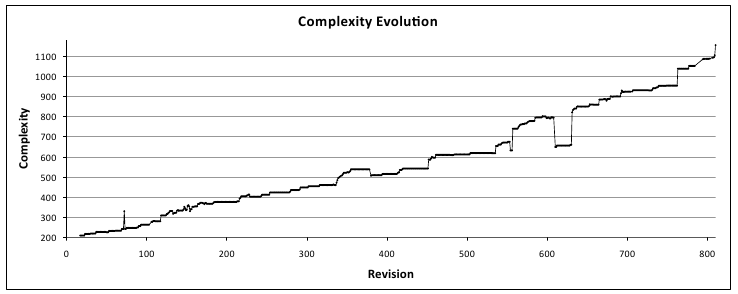
\includegraphics[width=1.00\textwidth]{img/cc-soetens.png}
	\end{frame}

	\begin{frame}
		\frametitle{Avaliação da ferramenta}
		\framesubtitle{Estudo original}
		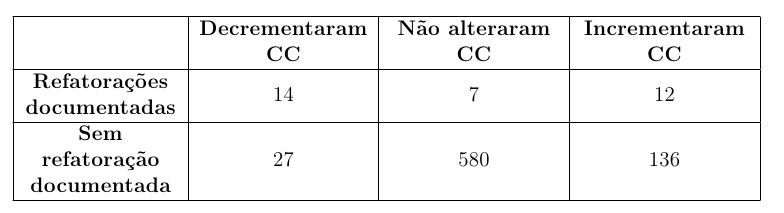
\includegraphics[width=1.00\textwidth]{img/tabela-soetens.png}
	\end{frame}

	\begin{frame}
		\frametitle{Avaliação da ferramenta}
		\framesubtitle{Análise dos autores}
		\begin{itemize}
			\item Poucas refatorações com remoção de código duplicado
			\item Commits com refatoração + nova funcionalidade
			\item Pequenas mudanças como movimentação de métodos e variáveis
		\end{itemize}
	\end{frame}

	\begin{frame}
		\frametitle{Avaliação da ferramenta}
		\framesubtitle{Reprodução do estudo}
		Consulta pela interface web\footnote{\url{http://metricminer.org.br/query/1}}
		Programa auxiliar para processar csv
		\begin{itemize}
			\item 250 projetos java
			\item 500 mil commits processados
		\end{itemize}
	\end{frame}

	\begin{frame}
		\frametitle{Avaliação da ferramenta}
		\framesubtitle{Reprodução do estudo}
		\begin{figure}[ht]
		\centering
		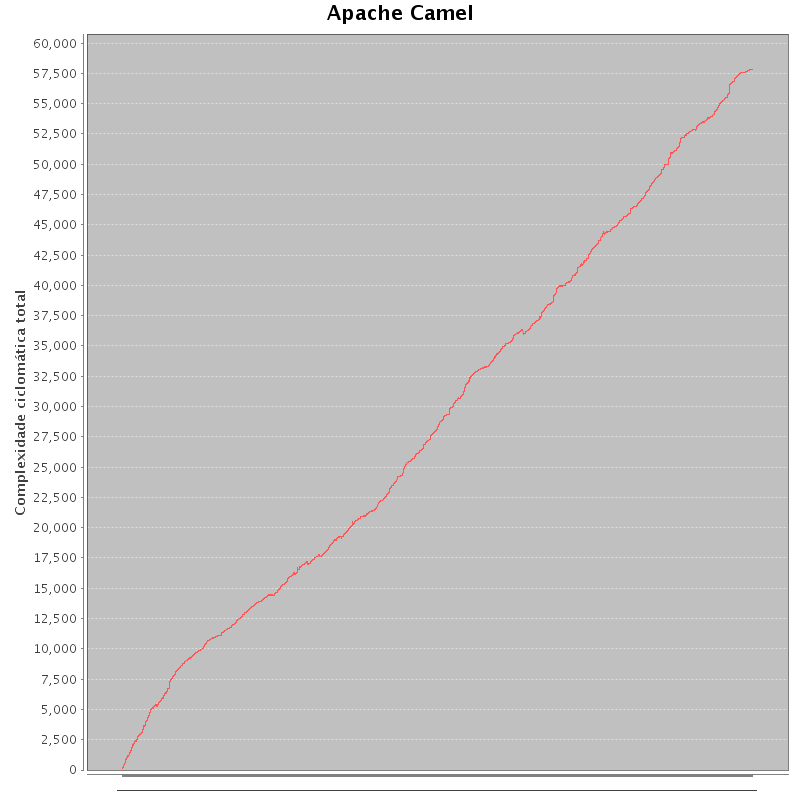
\includegraphics[width=0.7\textwidth]{img/camel.png}
		\end{figure}
	\end{frame}


	\begin{frame}
		\frametitle{Avaliação da ferramenta}
		\framesubtitle{Reprodução do estudo}
		\begin{figure}[ht]
		\centering
		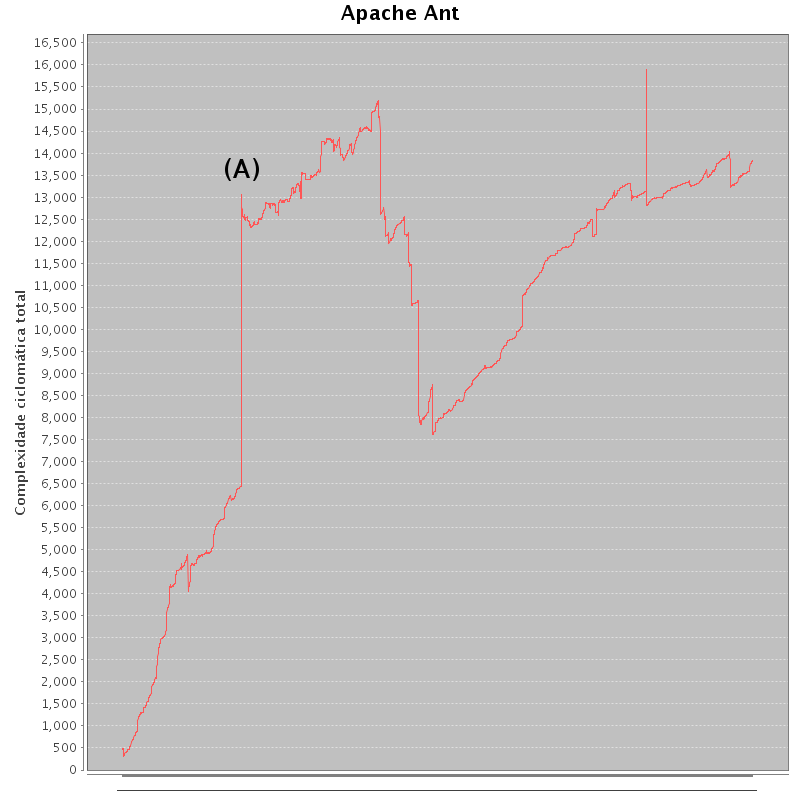
\includegraphics[width=0.7\textwidth]{img/ant.png}
		\end{figure}
	\end{frame}

	\begin{frame}
		\frametitle{Avaliação da ferramenta}
		\framesubtitle{Reprodução do estudo}
		\begin{figure}[ht]
		\centering
		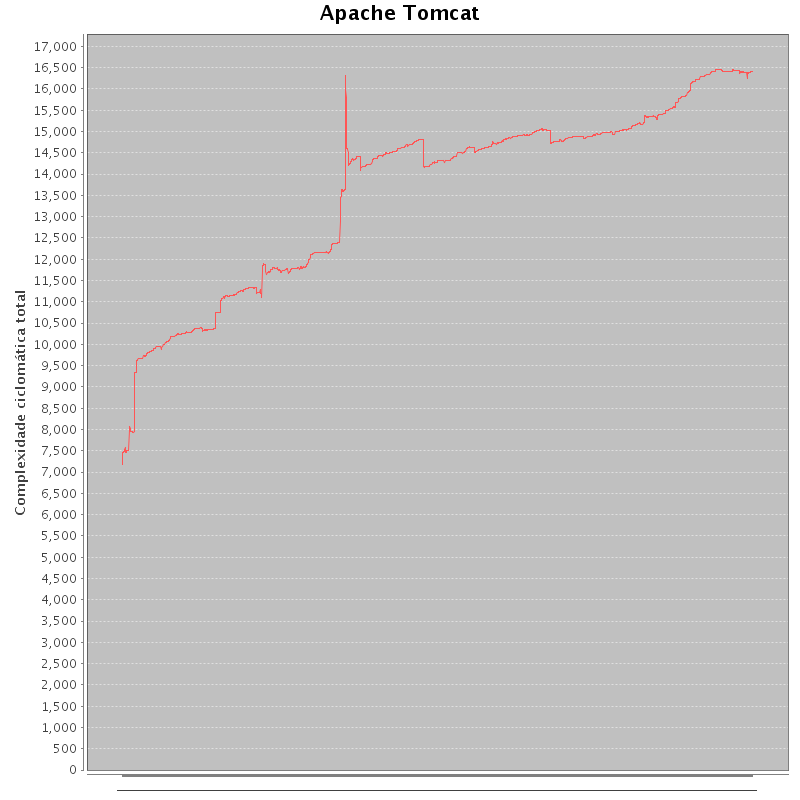
\includegraphics[width=0.7\textwidth]{img/tomcat.png}
		\end{figure}
	\end{frame}

	\begin{frame}
		\frametitle{Avaliação da ferramenta}
		\framesubtitle{Reprodução do estudo}
		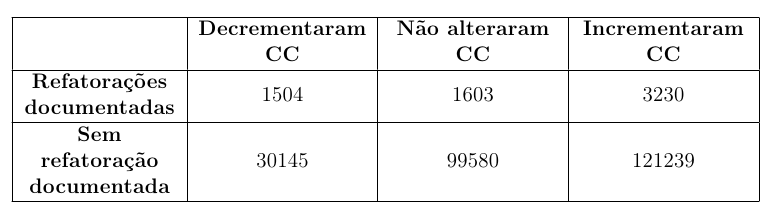
\includegraphics[width=1.00\textwidth]{img/tabela-metricminer.png}
	\end{frame}

	\begin{frame}
		\frametitle{Avaliação da ferramenta}
		\framesubtitle{Conclusão}
		\begin{itemize}
			\item Maior quantidade e variedade de projetos analisados
			\item Resultados semelhantes ao do estudo original
			\item Processo de mineração mais simples e eficiente
		\end{itemize}
	\end{frame}

	\begin{frame}
		\frametitle{Trabalhos futuros}
		\begin{itemize}
			\item Paralelizar
			\item Usabilidade da interface web
			\item Outras métricas e linguagens
			\item Sistemas de bug tracking, listas de email
			\item API
		\end{itemize}
	\end{frame}

	\begin{frame}
		\centering \Huge \textbf Obrigado!\\ \vspace{0.5cm}
		\centering \huge \textbf Perguntas?\\
	\end{frame}


% etc

\bibliographystyle{sbc}
\bibliography{apresentacao}
\end{document}